\section{Capacitores}

\subsection{Definición de capacitor}

Un capacitor\footnote{También conocido como condensador}, es un componente eléctrico pasivo que tiene la capacidad de almacenar energía en forma de un campo eléctrico. Está compuesto por dos conductores llamados placas separados por un material dieléctrico, que actúa como aislante.

Cuando se aplica una diferencia de potencial \(\Delta V\) entre las placas, una de ellas acumula carga positiva y la otra carga negativa, generando así un campo eléctrico entre ellas (ver figura \ref{fig:capacitor_charge}). La capacidad del capacitor para almacenar carga depende de sus características físicas y del dieléctrico utilizado.

\begin{figure}[!ht]
  \centering
  \begin{subfigure}[b]{.3\textwidth}
  \centering
  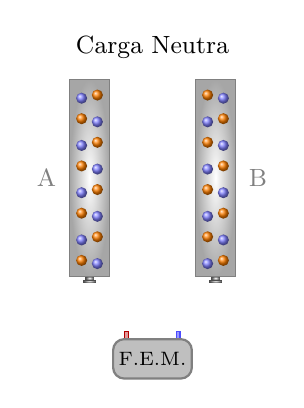
\begin{tikzpicture}
    \shade[inner color=white,outer color=black!70] (-.85,0) rectangle (-.75,-.05);
    \shade[inner color=white,outer color=black!70] (-.88,-.05) rectangle (-.72,-.08);

    \shade[inner color=white,outer color=black!70] (.85,0) rectangle (.75,-.05);
    \shade[inner color=white,outer color=black!70] (.88,-.05) rectangle (.72,-.08);

    \shadedraw[inner color=white,outer color=gray!70,color=gray] (-1.05,0) rectangle node[left=3mm] {\small A} (-0.55,2.5);
    \shadedraw[inner color=white,outer color=gray!70,color=gray] (1.05,0) rectangle node[right=3mm] {\small B} (0.55,2.5);
    \node at (0,2.9) {\small Carga Neutra};

    \filldraw[color=red!70!black,fill=red!70!black!40] (-.35,-.8) rectangle (-.3,-0.7);
    \filldraw[color=blue!70,fill=blue!40] (.35,-.8) rectangle (.3,-0.7);
    \filldraw[thick,color=gray,fill=gray!50,rounded corners] (-.5,-1.3) rectangle node {\color{black}\scriptsize F.E.M.} (.5,-0.8);

    \foreach \x\y in {.7/2.3,.9/2,.7/1.7,.9/1.4,.7/1.1,.9/.8,.7/.5,.9/.2} {
      \shade[ball color=orange] (\x,\y) circle (2pt);
      \shade[ball color=orange] (-\x,\y) circle (2pt);
    }

    \foreach \x\y in {.9/2.26,.7/1.96,.9/1.66,.7/1.36,.9/1.06,.7/.76,.9/.46,.7/.16} {
      \shade[ball color=blue!50] (\x,\y) circle (2pt);
      \shade[ball color=blue!50] (-\x,\y) circle (2pt);
    }
  \end{tikzpicture}
\end{subfigure}
\hfill 
\begin{subfigure}[b]{.3\textwidth}
  \centering
  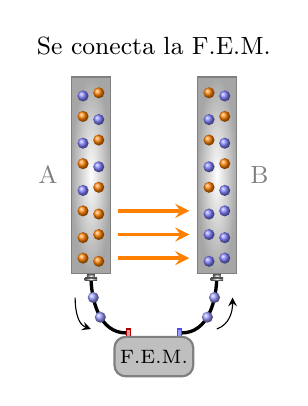
\begin{tikzpicture}[>=stealth]
    \draw[very thick] (-.8,0) to[out=270,in=180] (-.35,-.75);
    \shade[inner color=white,outer color=black!70] (-.85,0) rectangle (-.75,-.05);
    \shade[inner color=white,outer color=black!70] (-.88,-.05) rectangle (-.72,-.08);

    \draw[very thick] (.8,0) to[out=270,in=0] (.35,-.75);
    \shade[inner color=white,outer color=black!70] (.85,0) rectangle (.75,-.05);
    \shade[inner color=white,outer color=black!70] (.88,-.05) rectangle (.72,-.08);

    \draw[->] (-1,-.3) to[out=270,in=160] (-.8,-.7);
    \draw[<-] (1,-.3) to[out=270,in=20] (.8,-.7);
  
    \foreach \x\y in {.77/-.3,.68/-.55} {
      \shade[ball color=blue!40] (\x,\y) circle (2pt);
      \shade[ball color=blue!40] (-\x,\y) circle (2pt);
    }

    \shadedraw[inner color=white,outer color=gray!70,color=gray] (-1.05,0) rectangle node[left=3mm] {\small A} (-0.55,2.5);
    \shadedraw[inner color=white,outer color=gray!70,color=gray] (1.05,0) rectangle node[right=3mm] {\small B} (0.55,2.5);
    \node at (0,2.9) {\small Se conecta la F.E.M.};

    \filldraw[color=red!70!black,fill=red!70!black!40] (-.35,-.8) rectangle (-.3,-0.7);
    \filldraw[color=blue!70,fill=blue!40] (.35,-.8) rectangle (.3,-0.7);
    \filldraw[thick,color=gray,fill=gray!50,rounded corners] (-.5,-1.3) rectangle node {\color{black}\scriptsize F.E.M.} (.5,-0.8);

    \foreach \x\y in {.7/2.3,.9/2,.7/1.7,.9/1.4,.7/1.1} {
      \shade[ball color=orange] (\x,\y) circle (2pt);
      \shade[ball color=orange] (-\x,\y) circle (2pt);
    }
    \foreach \x\y in {.9/.8,.7/.5,.9/.2} {
      \shade[ball color=blue!50] (\x,\y) circle (2pt);
      \shade[ball color=orange] (-\x,\y) circle (2pt);
    }

    \foreach \x\y in {.9/2.26,.7/1.96,.9/1.66,.7/1.36,.9/1.06} {
      \shade[ball color=blue!50] (\x,\y) circle (2pt);
      \shade[ball color=blue!50] (-\x,\y) circle (2pt);
    }
    \foreach \x\y in {.7/.76,.9/.46,.7/.16} {
      \shade[ball color=blue!50] (\x,\y) circle (2pt);
      \shade[ball color=orange] (-\x,\y) circle (2pt);
    }
    \foreach \y in {.2,.5,.8} {
      \draw[very thick,orange,->] (-.45,\y) -- (.45,\y);
    }
  \end{tikzpicture}
\end{subfigure}
\hfill 
\begin{subfigure}[b]{.3\textwidth}
  \centering
  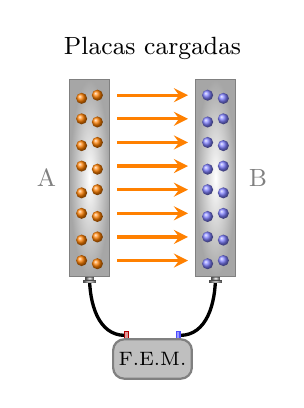
\begin{tikzpicture}[>=stealth]
    \draw[very thick] (-.8,0) to[out=270,in=180] (-.35,-.75);
    \shade[inner color=white,outer color=black!70] (-.85,0) rectangle (-.75,-.05);
    \shade[inner color=white,outer color=black!70] (-.88,-.05) rectangle (-.72,-.08);

    \draw[very thick] (.8,0) to[out=270,in=0] (.35,-.75);
    \shade[inner color=white,outer color=black!70] (.85,0) rectangle (.75,-.05);
    \shade[inner color=white,outer color=black!70] (.88,-.05) rectangle (.72,-.08);

    \shadedraw[inner color=white,outer color=gray!70,color=gray] (-1.05,0) rectangle node[left=3mm] {\small A} (-0.55,2.5);
    \shadedraw[inner color=white,outer color=gray!70,color=gray] (1.05,0) rectangle node[right=3mm] {\small B} (0.55,2.5);
    \node at (0,2.9) {\small Placas cargadas};

    \filldraw[color=red!70!black,fill=red!70!black!40] (-.35,-.8) rectangle (-.3,-0.7);
    \filldraw[color=blue!70,fill=blue!40] (.35,-.8) rectangle (.3,-0.7);
    \filldraw[thick,color=gray,fill=gray!50,rounded corners] (-.5,-1.3) rectangle node {\color{black}\scriptsize F.E.M.} (.5,-0.8);

    \foreach \x\y in {.7/2.3,.9/2,.7/1.7,.9/1.4,.7/1.1,.9/.8,.7/.5,.9/.2} {
      \shade[ball color=blue!50] (\x,\y) circle (2pt);
      \shade[ball color=orange] (-\x,\y) circle (2pt);
    }

    \foreach \x\y in {.9/2.26,.7/1.96,.9/1.66,.7/1.36,.9/1.06,.7/.76,.9/.46,.7/.16} {
      \shade[ball color=blue!50] (\x,\y) circle (2pt);
      \shade[ball color=orange] (-\x,\y) circle (2pt);
    }

    \foreach \y in {.2,.5,...,2.6} {
      \draw[very thick,orange,->] (-.45,\y) -- (.45,\y);
    }
  \end{tikzpicture}
\end{subfigure}

  \caption{Las cargas negativas fluyen de la placa A a la B.}
  \label{fig:capacitor_charge}
\end{figure}

\begin{definition}[Capacitancia]\label{def_capacitor}
La capacitancia \( C \) de un capacitor se define como la razón entre la magnitud de la carga \( Q \) almacenada en una de sus placas y la diferencia de potencial \( \Delta V \) entre las placas:
\begin{equation}
  C = \frac{Q}{V} ~[\unit{\farad}]
  \label{eq_definicion_capacidad}
\end{equation}
donde la capacitancia se mide en faradios y siempre es una cantidad positiva. 
\end{definition}

Un faradio es una unidad muy grande, por lo que en la práctica suelen utilizarse submúltiplos como el microfaradio (\unit{\micro\farad}), nanofaradio (\unit{\nano\farad}) o picofaradio (\unit{\pico\farad}).

La ecuación \eqref{eq_definicion_capacidad} de la definición \ref{def_capacitor} asume que las placas tienen cargas iguales y opuestas (\( +Q \) y \( -Q \)). Si el capacitor está desbalanceado, la capacitancia no puede obtenerse directamente con esta fórmula, pues el sistema ya no es un capacitor ideal y se requiere un análisis de campos más complejo. En la práctica el balance de carga entre placas se logra utilizando placas de dimensiones muy similares, de tal forma que la diferencia de cargas sea la mínima posible.

\subsection{Geometría de los conductores}

Sorprendentemente, a pesar de la definición \ref{def_capacitor}, en la práctica y durante la construcción de un capacitor la capacitancia total no depende de \(Q\) ni de la diferencia de potencial \(\Delta V\) entre sus placas, sino de la geometría del las placas y del material dieléctrico entre ellas. 

A continuación se listan los tipos geométricos de placas más comunes.

\subsubsection{1. Capacitor de placas planas paralelas}

Si se tienen placas paralelas, la capacidad depende de factores como el área \(A\) de las placas, la distancia \(d\) entre ellas y la permitividad \(\varepsilon\) del dieléctrico según la siguiente fórmula:
\[
C = \varepsilon \frac{A}{d}
\]
El parámetro \(\varepsilon\) del dieléctrico evidentemente depende del tipo de dieléctrico utilizado. Este parámetro es el ya mencionado valor de permitividad dieléctrica del material y se mide en \unit{\farad\per\meter} (faradios por metro).

\subsubsection{2. Capacitor esférico}

Consiste en dos esferas concéntricas de radios \( R_1 \) (interna) y \( R_2 \) (externa). Su capacitancia es:
\[
C = 4\pi \varepsilon_0 \frac{R_1 R_2}{R_2 - R_1}
\]

\subsubsection{3. Capacitor cilíndrico}

Está formado por dos cilindros coaxiales, uno de radio interno \( a \) y otro de radio externo \( b \), y de longitud \( L \) (suponiendo \( L \gg b \)). La capacitancia es:
\[
C = \frac{2\pi \varepsilon_0 L}{\ln(b/a)}
\]

\subsubsection{4. Geometrías irregulares o generales}

En geometrías más complejas, la capacitancia no puede obtenerse de forma analítica sencilla. En estos casos se recurre a aproximaciones por métodos numéricos o bien por aproximaciones analíticas. En general, se busca construir capacitores con formas sencillas. Por otro lado, los ejercicios de capacitores y capacidad no pretenden encontrar la capacidad de una geometría irregular.

\subsection{Energía almacenada en un capacitor}

La fórmula de la energía almacenada en un capacitor,
\begin{equation}
    U = \frac{1}{2} QV
\end{equation}
puede demostrarse considerando el trabajo necesario para cargar el capacitor, es decir, para mover carga desde una placa a la otra en contra del campo eléctrico generado.

Supongamos que inicialmente el capacitor no tiene carga. Para cargarlo, se debe transferir carga desde una placa hacia la otra (esto lo realizará una f.e.m). En un instante cualquiera, si la carga acumulada es \( q \), la diferencia de potencial entre las placas es:
\[
  V(q) = \frac{q}{C}
\]
Para mover una carga diferencial \( dq \) contra esta diferencia de potencial, se debe realizar un trabajo diferencial:
\[
  dW = V(q) \, dq = \frac{q}{C} \, dq
\]
Entonces, el trabajo total \( W \) para cargar el capacitor desde \( q = 0 \) hasta \( q = Q \) es:
\[
  W = \int_{0}^{Q} \frac{q}{C} \, dq = \frac{1}{C} \int_{0}^{Q} q \, dq = \frac{1}{C} \cdot \frac{Q^2}{2} = \frac{1}{2} \frac{Q^2}{C}
\]
Ese trabajo realizado es la energía almacenada en el campo eléctrico del capacitor, por lo tanto:
\[
  \boxed{U = \frac{1}{2} \frac{Q^2}{C}}
\]
Como \( Q = CV \), podemos reemplazar en la expresión para obtener las otras formas equivalentes de la energía. En función de \( Q \) y \( V \):
\[
  U = \frac{1}{2} QV
\]
y en función de \( C \) y \( V \):
\[
  U = \frac{1}{2} CV^2
\]
Estas tres expresiones son equivalentes, y se utilizan según las variables conocidas en un problema.

\begin{tcolorbox}[myconclusion]
La energía \( U \) no está en la carga como tal, sino en el sistema carga-campo eléctrico que se establece entre las placas del capacitor. Esta energía puede recuperarse, por ejemplo, al descargar el capacitor en un circuito.
\end{tcolorbox}

\subsection{Dieléctrico en un capacitor}

El dieléctrico es un material aislante que se coloca entre las placas de un capacitor. Su función principal es modificar el campo eléctrico dentro del capacitor y, como consecuencia, aumentar su capacitancia sin necesidad de cambiar su geometría.

\begin{figure}[ht]
    \centering
    \includegraphics[width=0.8\textwidth]{capacitor_dielectric.png}
    \caption{Polarización de un dieléctrico en un capacitor.}
    \label{fig_polarizacion_dielectrico}
\end{figure}
Cuando se introduce un dieléctrico entre las placas de un capacitor este se polariza, lo que significa que las moléculas del dieléctrico se alinean parcialmente con el campo eléctrico como se muestra en la figura \ref{fig_polarizacion_dielectrico}, creando campos eléctricos internos opuestos al campo aplicado. Esto reduce el campo eléctrico efectivo entre las placas, por tanto, para una misma cantidad de carga \( Q \), la diferencia de potencial \( V \) disminuye. Como \( C = Q/V \), un menor \( V \) implica una mayor capacitancia.

El efecto del dieléctrico se caracteriza mediante una constante adimensional llamada permitividad relativa o constante dieléctrica, denotada por:
\[
  \varepsilon_r = \mathcal{K} = \frac{\varepsilon}{\varepsilon_0} 
\]
donde \( \varepsilon_r = \mathcal{K} \) es la permitividad relativa del material dieléctrico y \( \varepsilon \) es la permitividad del material dieléctrico.

Algunas bibliografías utilizan la letra ``k cursiva'' (\textit{k}) para referirse a la constante dieléctrica. Aunque usar \( \varepsilon_r \) evita confusión con la constante \(k\) de la ley de Coulomb, en este texto se utilizará la letra ``k caligráfica'' \(\mathcal{K}\), de modo que se pueda distinguir con facilidad y mantener el estándar de notación.

Cuando se introduce un dieléctrico completamente entre las placas, la capacitancia del capacitor se modifica de:
\[
  C_0 = \varepsilon_0 \frac{A}{d}
  \quad \text{sin dieléctrico a} \quad
  C = \mathcal{K} \varepsilon_0 \frac{A}{d} = \varepsilon \frac{A}{d}
  \quad \text{con dieléctrico}
\]
Por lo tanto:
\begin{equation}
  \boxed{C = \mathcal{K} C_0}
  \label{eq:capacitance_dielectric}
\end{equation}

Esto significa que la capacitancia aumenta en un factor \( \mathcal{K} \), que típicamente está entre 2 y 10 para muchos materiales comunes, aunque puede ser mucho mayor en materiales especiales.

Experimentar con placas paralelas y diferentes dieléctricos permite evidenciar que no solo cambia su capacidad sino que la energía también cambia dependiendo de cómo se conecta el capacitor. Suponiendo un par de placas paralelas y vacío entre ellas, que no es más que un dieléctrico cuyo valor de permitividad es \(\varepsilon_0\), tomaremos otro material dieléctrico de valor \(\varepsilon\neq\varepsilon_0\) tal que su permitividad relativa es \(\mathcal{K}\) veces mayor que \(\varepsilon_0\).

\marginnote{
  \begin{tcolorbox}[sidenote]\small
    Cuidado, si se introduce un dieléctrico y \(C\) aumenta, es tentador pensar que \(U=1/2 ~ CV^2\) siempre aumenta al ver la expresión. Sin embargo recuerde que si no hay f.e.m conetada, \(V\) disminuye y la fórmula de la energía tiene un factor de potencial cuadrático. Consecuentemente como \(C\) es proporcional a \(V\) resulta que \(U<U_0\) lo cual es consistente con el experimento.
  \end{tcolorbox}
}
Considerando la situación entonces, si el capacitor está desconectado de la fuente con alguna cantidad de carga \(Q\) y se inserta el dieléctrico, entonces \( Q \) se mantiene constante, ya que esta desconectado de la fuente y no hay f.e.m que desplace cargas, por otro lado, \( V \) disminuye por que se reorientan los dipolos, y por tanto se forma un campo eléctrico opuesto en el dieléctrico y, por último, \( C \) aumenta, debido a la relación entre variables dada por la definición de capacidad (ecuación \ref{eq_definicion_capacidad}). Un importante detalle adicional es que la energía disminuye ya parte de la energía se transfiere al dieléctrico como trabajo de polarización.
\[
U = \frac{1}{2} \frac{Q^2}{C} \quad \text{(disminuye porque } C \text{ aumenta)}
\]

Otro escenario posible consiste en conectar el capacitor a una fuente de \( V \) constante y luego modificar su dieléctrico. Al insertar el dieléctrico, debido a las características de la fuente, \( V \) se mantiene constante, esto provoca que \( Q \) aumente, ya que la fuente desplaza nuevas cargas para mantener la diferencia de potencial entre las placas. Y al igual que en el caso anterior, \( C \) aumenta, pero en contraste, la energía almacenada aumenta, y esta energía adicional proviene de la fuente de tensión.
\[
U = \frac{1}{2} C V^2 \quad \text{(aumenta porque } C \text{ aumenta)}
\]

De estos experimentos se puede observar que el dieléctrico tiene varios efectos importantes en un capacitor. Aumenta la capacitancia \( C \) en un factor de \(\mathcal{K}\) veces la capacidad original. Reduce el campo eléctrico \( E \) entre las placas debido a que el dieléctrico genera un campo eléctrico opuesto y almacena energía adicional en forma de polarización. Debido a esto último modifica la energía almacenada \( U \) y cambia la expresión de capacitancia \( C \).
\begin{tcolorbox}[myconclusion]
  Un importante detalle es que si, se tiene un capacitor con su máxima carga y no está conectado a la fuente, al colocar el dieléctrico, por más de que aumente la capacidad \(C\) del capacitor, no se modifica la cantidad de carga \(Q\) almacenada en el mismo. Es decir, si habían \qty{4}{\micro\coulomb} de carga, entonces esos \qty{4}{\micro\coulomb} se mantendrán igual, pero ahora el capacitor puede aceptar más carga, es decir, tiene más espacio para alojar carga eléctrica.
\end{tcolorbox}

Un importante parámetro del dieléctrico es la llamada tensión de ruptura dieléctrica, que es la máxima diferencia de potencial que puede aplicarse entre las placas de un capacitor o entre dos puntos de un aislante antes de que el material dieléctrico falle y se vuelva conductor. Este parámetro generalmente se da inscripto en el propio capacitor, indicando su tensión nominal de funcionamiento y su tensión máxima de ruptura.

Cuando el campo eléctrico en el dieléctrico supera un valor crítico, llamado intensidad de campo de ruptura (o rigidez dieléctrica), el material se ioniza, es decir, sus átomos o moléculas pierden electrones debido al campo intenso, y se produce una descarga eléctrica: el dieléctrico pierde su capacidad aislante y permite el paso de corriente.

\subsection{Capacitores en serie y paralelo}

Los capacitores pueden conectarse en serie o en paralelo, y la forma en que se conectan afecta la capacitancia total del circuito.

\subsubsection{1. Capacitores en paralelo}

Se dice que los capacitores (o cualquier componente eléctrico) tiene una configuración en paralelo cuando se conecta tal y como se muestra en la figura \ref{fig:capacitors_parallel}.
\begin{figure}[!ht]
  \centering
  \includegraphics[width=0.8\textwidth]{capacitors_parallel.png}
  \caption{Configuración de capacitores en paralelo.}
  \label{fig:capacitors_parallel}    
\end{figure}

En definitiva, todos los capacitores están conectados a la misma diferencia de potencial \( V \). Es decir:
\[
  V_1 = V_2 = \dots = V_n = V
\]
La carga total almacenada es la suma de las cargas individuales:
\[
  Q_{\text{total}} = Q_1 + Q_2 + \dots + Q_n
\]
Como \( Q_i = C_i V \), entonces:
\[
  Q_{\text{total}} = C_1 V + C_2 V + \dots + C_n V = \left( C_1 + C_2 + \dots + C_n \right) V
\]
Pero, por definición:
\[
Q_{\text{total}} = C_{\text{eq}} V
\]
Comparando ambas expresiones:
\begin{equation}
    \boxed{C_{\text{eq}} = C_1 + C_2 + C_3 + \ldots + C_n}
\end{equation}
Cuando los capacitores están conectados en paralelo, la capacitancia equivalente \( C_{\text{eq}} \) se calcula sumando las capacitancias individuales.

\subsubsection{2. Capacitores en serie}

Se dice que los capacitores (o cualquier componente eléctrico) tiene una configuración en serie cuando se conecta tal y como se muestra en la figura \ref{fig:capacitors_series}.
\begin{figure}[!ht]
    \centering
    \includegraphics[width=0.9\textwidth]{capacitors_series.png}
    \caption{Configuración de capacitores en serie.}
    \label{fig:capacitors_series}
\end{figure}

Todos los capacitores están conectados uno tras otro, por lo tanto, se tendrá en todos los capacitores la misma carga \( Q \),
\[
Q_1 = Q_2 = \dots = Q_n = Q
\]
En definitiva, la cantidad de carga que el capacitor más pequeño pueda almacenar limitará al resto de capacitores. Resultando esto en tener todos la misma carga. Esto puede observarse en la figura \ref{fig:capacitors_series_charge}.
\begin{figure}[!ht]
    \centering
    \includegraphics[width=0.8\textwidth]{capacitor_series_charge.png}
    \caption{La carga en ambos capacitores es la misma.}
    \label{fig:capacitors_series_charge}
\end{figure}

Como se puede ver en la figura \ref{fig:capacitors_series_charge}, la carga en ambos capacitores es la misma porque el capacitor \(C_2\) (más pequeño) está completamente cargado, esto provoca que el capacitor \(C_1\) (más grande) se vea limitado y no se use toda la capacidad. Esto es así porque los electrones se mueven de la placa izquierda del capacitor \(C_1\) a la placa derecha del capacitor \(C_2\). Cuando el capacitor \(C_2\) se carga completamente no puede acumular más carga. Por otro lado el capacitor \(C_1\) aún tiene electrones en su placa izquierda, pero estos electrones no tienen a donde ir, por lo que no se puede acumular más carga. Lo mismo sucede en las placas del medio de ambos capacitores. En una configuración en serie, la carga del capacitor más pequeño será la carga total usada de la f.e.m.

Como la carga en todos los capacitores es la misma, la diferencia de potencial entre las placas de cada capacitor será diferente. La diferencia de potencial total es la suma de las diferencias de potencial individuales:
\[
  V_{\text{total}} = V_1 + V_2 + \dots + V_n
\]
Pero \( V_i = \frac{Q}{C_i} \), entonces:
\[
  V_{\text{total}} = \frac{Q}{C_1} + \frac{Q}{C_2} + \dots + \frac{Q}{C_n} = Q \left( \frac{1}{C_1} + \frac{1}{C_2} + \dots + \frac{1}{C_n} \right)
\]
Por definición, \( V_{\text{total}} = \frac{Q}{C_{\text{eq}}} \), así que:
\[
  \frac{Q}{C_{\text{eq}}} = Q \left( \frac{1}{C_1} + \frac{1}{C_2} + \dots + \frac{1}{C_n} \right)
\]
Dividiendo ambos lados por \( Q \neq 0 \):
\begin{equation}
  \boxed{\frac{1}{C_{\text{eq}}} = \frac{1}{C_1} + \frac{1}{C_2} + \frac{1}{C_3} + \ldots + \frac{1}{C_n}}
\end{equation}
Resultando que la inversa de la capacitancia equivalente en serie es igual a la suma de las inversas de las capacitancias individuales.
